\documentclass[12pt]{article}
	
\title{CSC 320 - Worksheet 4}
\author{Nadeem Abdul Hamid}
\date{January 23, 2024}  


\usepackage[margin=1in]{geometry}		% For setting margins
\usepackage{amsmath}				% For Math
\usepackage{amsthm}
\usepackage{fancyhdr}				% For fancy header/footer
\usepackage{graphicx}				% For including figure/image
\usepackage{cancel}					% To use the slash to cancel out stuff in work
\usepackage[shortlabels]{enumitem}
\usepackage{hyperref}
\usepackage{jigsaw}

\usepackage{algorithm,caption}
\usepackage{algpseudocodex}
% docs: https://ctan.math.washington.edu/tex-archive/macros/latex/contrib/algpseudocodex/algpseudocodex.pdf


%%%%%%%%%%%%%%%%%%%%%%
% Set up fancy header/footer
% taken from https://www.overleaf.com/latex/templates/homework-template/yvgnmrbywwnp
\makeatletter    % for \@ in \@title
\pagestyle{fancy}
\fancyhead[LO,L]{\@author}
\fancyhead[CO,C]{\@title}
\fancyhead[RO,R]{\@date}
\fancyfoot[LO,L]{}
\fancyfoot[CO,C]{\thepage}
\fancyfoot[RO,R]{}
\renewcommand{\headrulewidth}{0.4pt}
\renewcommand{\footrulewidth}{0.4pt}
\makeatother    % restore
%%%%%%%%%%%%%%%%%%%%%%


%%%%%%%%%%%%%%%%%%%%%%
% from: https://tex.stackexchange.com/questions/14667/does-latex-define-a-semantic-equivalent-of-textbf
\makeatletter
\newcommand{\strong}[1]{\@strong{#1}}
\newcommand{\@@strong}[1]{\textbf{\let\@strong\@@@strong#1}}
\newcommand{\@@@strong}[1]{\textnormal{\let\@strong\@@strong#1}}
\let\@strong\@@strong
\makeatother
%%%%%%%%%%%%%%%%%%%%%%


\newcommand{\emptybox}[2][\textwidth]{%
  \begingroup
  \setlength{\fboxsep}{-\fboxrule}%
  \noindent\framebox[#1]{\rule{0pt}{#2}}%
  \endgroup
}

\newtheorem{theorem}{Theorem}
\newtheorem{lemma}{Lemma}


\begin{document}

\section{Recursion (Sorting/Selection)}

\subsection{Counting Inversions}

Which of these arrays is more ``sorted"?\\~

\begin{minipage}{0.5\textwidth}\centering
\begin{tabular}{|*{7}{c|}}
    \hline
    15 & 8 & 23 & 5 & 29 & 12 & 4 \\
    \hline
  \end{tabular}
\end{minipage}%
\begin{minipage}{0.5\textwidth}\centering
  \begin{tabular}{|*{7}{c|}}
    \hline
    4 & 8 & 5 & 12 & 23 & 29 & 15 \\
    \hline
  \end{tabular}
\end{minipage}%
  
\vspace{1in}

\begin{minipage}{0.5\textwidth}\centering
    \begin{tabular}{|*{7}{c|}}
        \hline
        ~~~  & ~~~  & ~~~ & ~~~ & ~~~ & ~~~ & ~~~ \\
        ~~~  & ~~~  & ~~~ & ~~~ & ~~~ & ~~~ & ~~~ \\
        \hline
      \end{tabular}
    \end{minipage}%
    \begin{minipage}{0.5\textwidth}\centering
      \begin{tabular}{|*{7}{c|}}
        \hline
        ~~~  & ~~~  & ~~~ & ~~~ & ~~~ & ~~~ & ~~~ \\
        ~~~  & ~~~  & ~~~ & ~~~ & ~~~ & ~~~ & ~~~ \\
        \hline
      \end{tabular}
    \end{minipage}% 
\\~

Write out a sorted copy of the array in each of the blank tables here. Draw lines from each number in the mixed up list to the corresponding number in the sorted list. What do you notice about these lines? What does that represent?

\vspace{1in}

Define:

\begin{quote}
    An \textbf{inversion} in an array $A[1..n]$ is a pair of indices $(i, j)$ such that:
\end{quote}

\vspace{1in}

\begin{minipage}{0.5\textwidth}\centering
    What array of size $n$ has the largest number of inversions, and what is that number? (Assume distinct elements for simplicity.)
\end{minipage}%
\begin{minipage}{0.5\textwidth}\centering
    What array has the smallest number of inversions?
\end{minipage}% 
\\~


\clearpage
\subsubsection*{Brute Force Algorithm}

Describe a straightforward, brute-force algorithm to count the number of inversions in an array.

\begin{algorithmic}
    \Procedure{CountInversionsBF}{$A[1..n]$}
    \LComment{Input: an array of integers \\
              Output: the number of pairs of integers in the array that are out of order.\\}

    \LComment{\vspace{2in}}

    \EndProcedure
\end{algorithmic}

What is the time complexity of this?


\subsubsection*{Recursive (Divide-and-conquer)}

Describe a recursive algorithm that splits the array into equal halves and recursively finds the inversion counts and then calculates the overall count somehow.

\begin{algorithmic}
    \Procedure{CountInversionsRec}{$A[1..n], i, j$}
    \LComment{Input: an array of integers, and indices of a subsection of the array, $A[i..j]$ \\
              Output: the number of pairs of integers in A[i..j] that are out of order.\\}

    \LComment{\vspace{2.25in}}

    \EndProcedure
\end{algorithmic}

What is the time complexity of this?\footnote{What about the space complexity?}  \\(Write a recurrence relation and use the Master Theorem.) 



\subsubsection*{Smarter Recursive (Divide-and-conquer)}

\begin{quote}
\it The trick to making divide-and-conquer efficient is to make it so that
conquering is easier than just solving the whole problem.
\end{quote}

\begin{itemize}
    \item Fix some $i$ on the left side. How many $j$ on the right side form
    inversions?\\~ 

    \begin{minipage}{0.5\textwidth}\centering
        \begin{tabular}{|*{5}{c|}}
            \hline
            8 & 2 & 91 & 22 & 57 \\
            \hline
            $\uparrow$ \\
            $i$
          \end{tabular}
        \end{minipage}%
        \begin{minipage}{0.5\textwidth}\centering
          \begin{tabular}{|*{5}{c|}}
            \hline
            6 & 10 & 1 & 7 & 4 \\
            \hline 
           \end{tabular}
           \\~\\~
        \end{minipage}%
    \vspace{.25in}    

    \item What would we do if the right hand side were sorted?\\~

    \begin{minipage}{0.5\textwidth}\centering
        \begin{tabular}{|*{5}{c|}}
        \hline
        8 & 2 & 91 & 22 & 57 \\
        \hline
        $\uparrow$ \\
        $i$
      \end{tabular}
    \end{minipage}%
    \begin{minipage}{0.5\textwidth}\centering
      \begin{tabular}{|*{5}{c|}}
        \hline
        1 & 4 & 6 & 7 & 10 \\
        \hline
       \end{tabular}
       \\~\\~
    \end{minipage}%
    \vspace{.25in}    
    
    \item Time?
    \vspace{.5in}    
    
    \item So... what's the problem with presorting? 
    \vspace{.5in}    
    
    \item Ok, sort (both halves of the array) as part of the process...

    \item Count the total number of inversions between elements in these two halves of an array:
    
    \begin{minipage}{0.5\textwidth}\centering
        \begin{tabular}{|*{5}{c|}}
            \hline
            2 & 8 & 22 & 57 & 91 \\
            \hline
            $\uparrow$ \\
            $i$
          \end{tabular}
        \end{minipage}%
        \begin{minipage}{0.5\textwidth}\centering
          \begin{tabular}{|*{5}{c|}}
            \hline
            1 & 4 & 6 & 7 & 10 \\
            \hline
            $\uparrow$ \\
            $j$
          \end{tabular}
        \end{minipage}%
        \vspace{1in}    
            
    \item Does this feel familiar?
    
\end{itemize}

Modify merge sort\dots

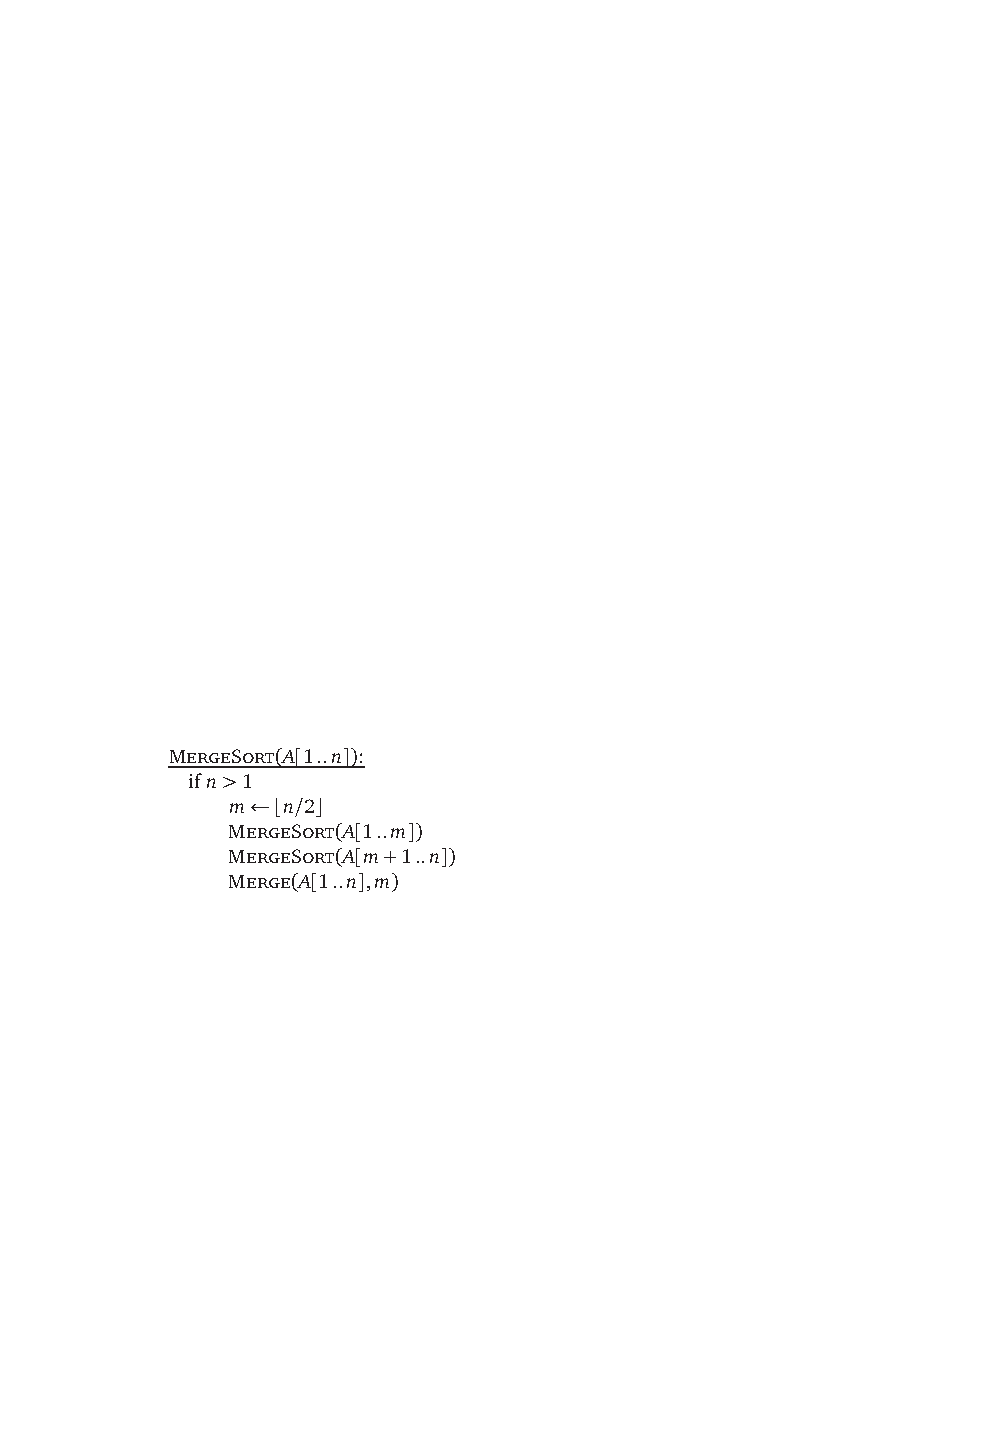
\includegraphics[scale=1.5]{w04-mergesort.pdf}\\~

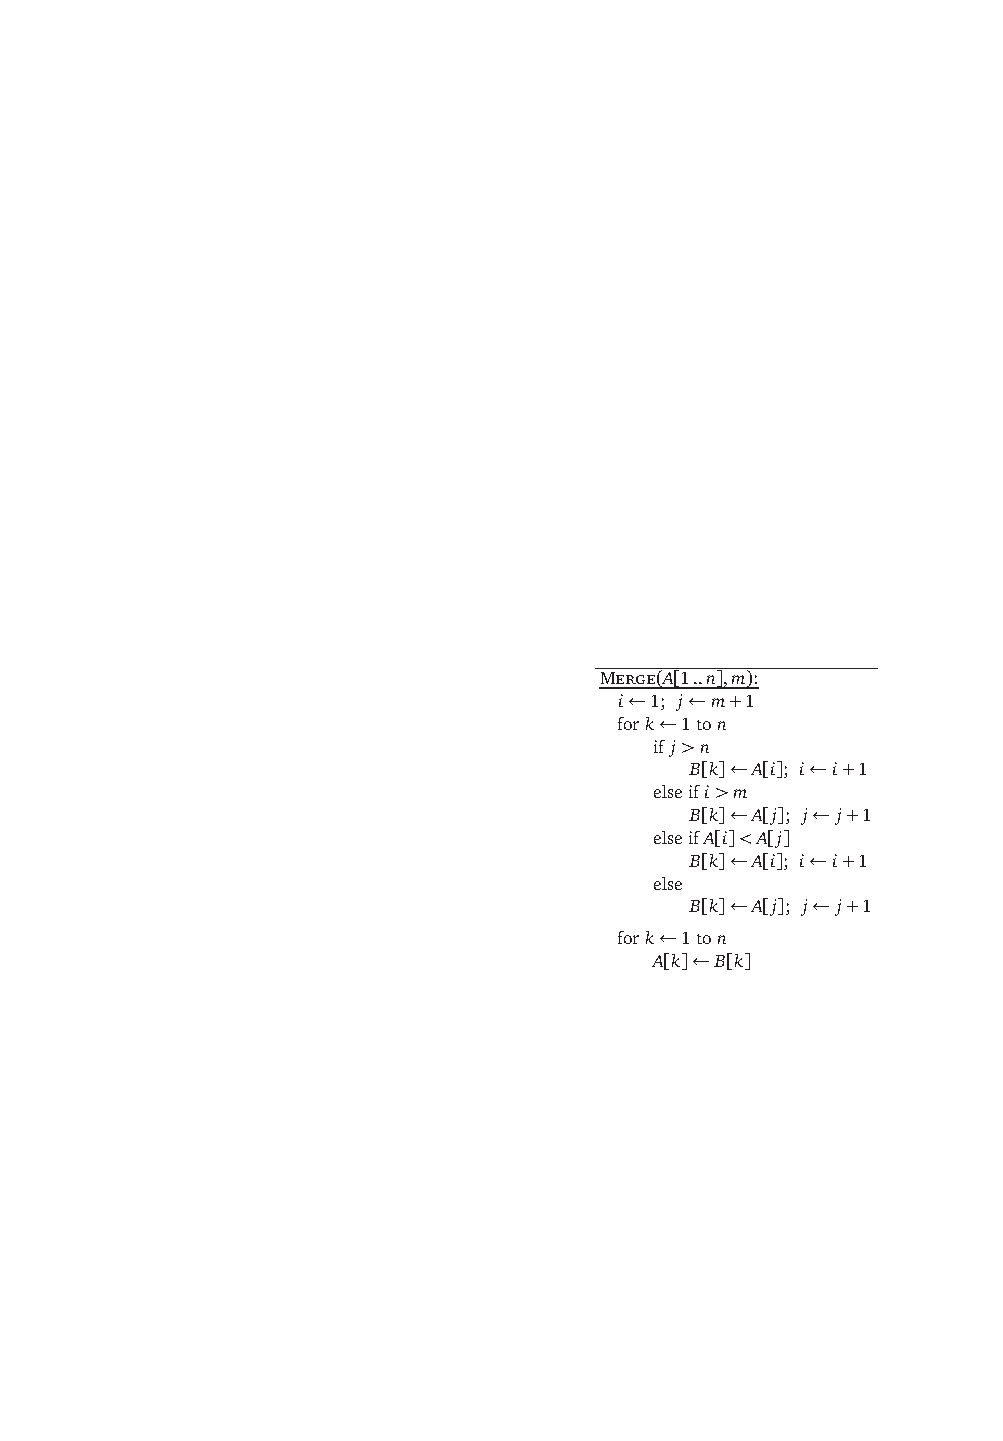
\includegraphics[scale=1.75]{w04-merge.pdf}

\vspace{.5in}
\noindent Prove the number of inversions (assume an array of length $2^k$) is correctly counted.



\end{document}



